\documentclass[a4paper,12pt]{article}
\usepackage{graphicx}
\usepackage[left=30mm, right=30mm, top=30mm, bottom=30mm]{geometry}
\usepackage{amsmath}
\usepackage{siunitx}
\usepackage{fancyhdr}
\usepackage{url}
\pagestyle{fancy}
%-------------------------------------------------------------------------------
\lhead{\textbf{CE394M}}
\rhead{\textbf{Advanced Analysis in Geotechnical Engineering}}
\cfoot{\thepage}
%-------------------------------------------------------------------------------

\begin{document}
\begin{centering}
	\textbf{
		Assignment 7b: Bearing capacity of drained sands
	}
\end{centering}

\vspace{1em}
\begin{figure}[!h]
	\centering
	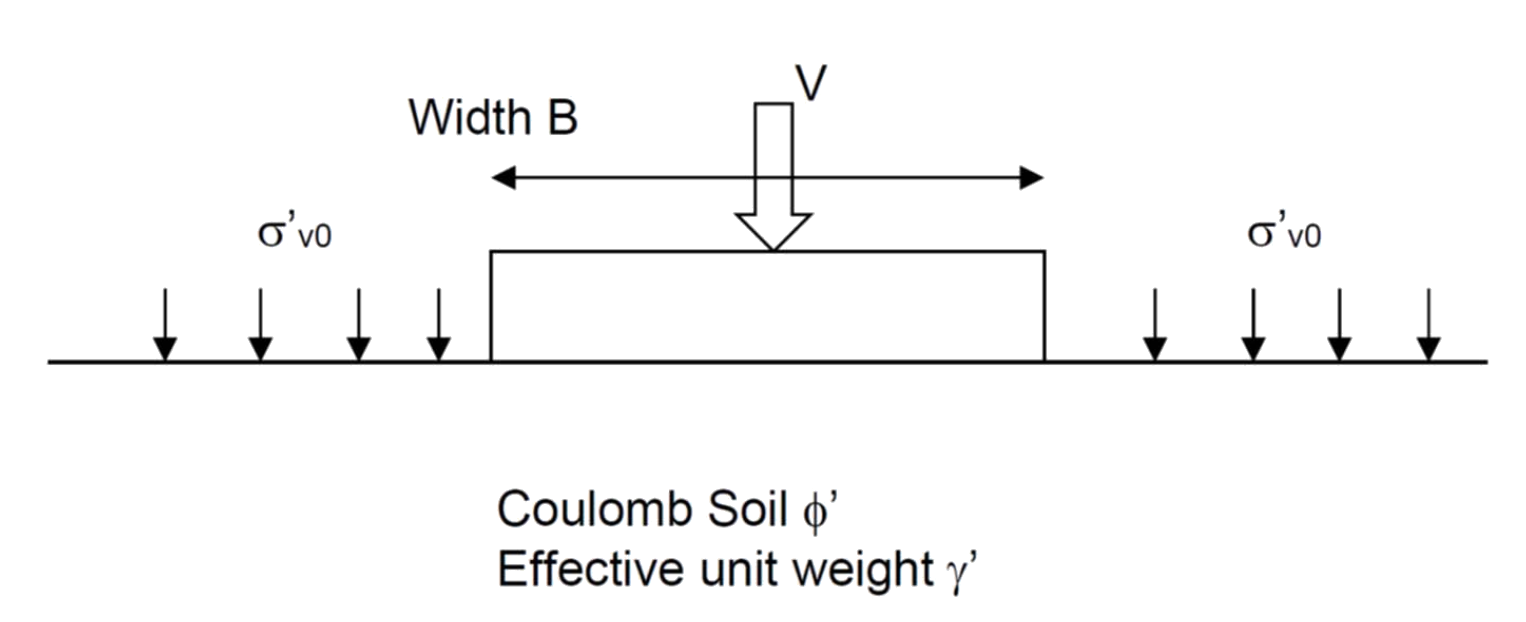
\includegraphics[width=0.85\textwidth]{figs/bearing-capacity.png}
\end{figure}
 
The bearing capacity of drained sand is defined as:

\begin{align*}
q_f = V/B = 0.5 N_\gamma \gamma^\prime B + N_q \sigma_{v0}^\prime \\
\end{align*}
$0.5 N_\gamma \gamma^\prime B $ is the resistance due to confinement of the soil. $N_q \sigma_{v0}^\prime$ is the resistance due to the surcharge. 

However, the bearing capacity evaluated using the above equation is incorrect. Using the specific example shown below, prove that the classical superposition solution of resistance due to confinement of the soil + resistance due to surcharge is conservative. To solve the bearing capacity equation, you may want to use the Analysis of Bearing Capacity software~\url{http://www2.eng.ox.ac.uk/civil/people/cmm/software}.  Unfortunately this only works on Windows, please let me know if you have any issues.

A 5 m wide rough strip footing on Coulomb dry soil with a density of $20 kN/m^3$, friction angle LaTeX: $\phi=30\deg$, and a surcharge of $10 kN/m^2$. Evaluate the following: 

Additional reading material: Determination of bearing capacity of shallow foundations without using superposition approximation.

\begin{enumerate}
\item Bearing capacity purely due to the confinement of the soil (kPa): %738
\item Bearing capacity purely due to surcharge (ignore resistance due to soil confinement) in kPa: %184
\item Bearing capacity of drained sand (combined effect based on the above equation) in kPa: %921.7
\item Numerical solution using the Analysis of Bearing Capacity (software) for the combined effect of self-weight and surcharge in (kPa): %1084.8
  \item Discuss your results and explain why a difference is observed between the bearing capacity equation and the numerical solution?

%The bearing capacity equations widely available rely on Terzaghi's superposition assumption which is considered conservative and would always result in a safer design.

%However, ABC software uses what is classified as 'partial' or 'incomplete' lower-bound collapse load which only calculates part of the stress field at collapse, which is needed to compute the bearing capacity. This method of calculating stress field for Mohr-coulomb materials is only accurate if the dilation angle is equal to the friction angle which is only valid when the soil undergoes undrained behavior. Because this method does not rely on superposition and considers the effect of overburden and confinement simultaneously, it will result in a higher estimate of bearing capacity which is a lower bound for the true solution and can match it under certain conditions.

  \end{enumerate}
\end{document}

